% !TEX root = Bachelorarbeit Synthetische Daten.tex
\chapter{Methodisches Vorgehen}

In diesem Kapitel wird das methodische Vorgehen der Arbeit beschrieben.

\section{MVIP-Datensatz} \label{sec:dataset}

% EIBA-Artikel: \parencite{ReziProK2019eiba}
% MVIP-Datensatz: \parencite{Koch2023mvip}

...

\subsection{Teildatensatz} \label{sec:subdataset}

% Wahl eines Teildatensatzes mit 20 "CarComponent" Klassen
Um die Rechenzeit zu reduzieren und die Experimente auf eine bestimmte Objektkategorie zu beschränken, wurde ein Teildatensatz des EIBA-Datensatzes verwendet. Dabei wurden zufällig 20 Klassen aus der super class "CarComponent" ausgewählt. Es wurden außerdem nur die RGB-Bilder verwendet, allerdings kommen auch die Objektmasken im Pre-Processing der Daten zum Einsatz. ...

% Details: Klassen und Anzahl der Bilder in Teildatensatz
Der Teildatensatz enthält insgesamt ... Bilder, die in ... Klassen eingeteilt sind. Die Klassen sind ungleichmäßig verteilt, wobei einige Klassen nur wenige Bilder enthalten, während andere sehr viele Bilder haben. ...

% Beispielbilder, -masken
\begin{figure}
	\centering
	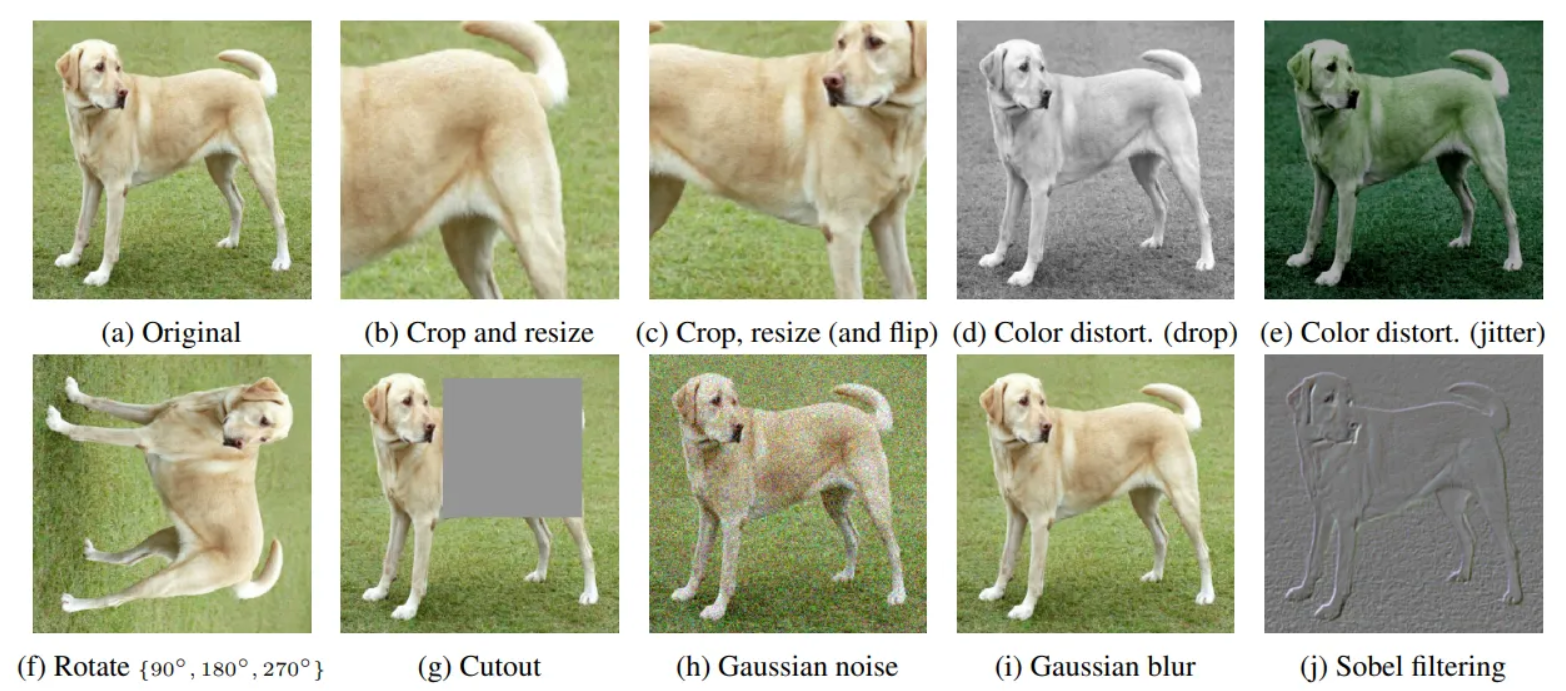
\includegraphics[width=\textwidth]{figure_data_augmentation.png}
	\caption{Beispielbilder aus dem MVIP-Teildatensatz.}
\end{figure}

\subsection{Vorverarbeitung} \label{sec:preprocessing}

% Verwendung der Objektmasken, um die Bilder zu croppen
	% Bounding Box
	% Quadratischer Output
	% Weniger Aufmerksamkeit auf gleichbleibenden Hintergrund
% Verschiedene "klassische" Augmentationen
	% Rotation
	% ColorJitter
% Normalisierung der Bilder
...

\section{Implementierung} \label{sec:implementation}

% Arbeitsumgebung, Rechner-Zugang, etc.
% Verwendung vorhandener Implementierungen
% Gemeinsame Programmiersprache, Bibliotheken, etc.

Für die Vorbereitung der in dieser Arbeit durchgeführten Experimente konnte sich größtenteils auf die Implementierung von DA-Fusion und Supervised Contrastive Learning aus den Quellen ... und ... gestützt werden. Beide Implementierungen sind in Python geschrieben und verwenden die Bibliothek PyTorch. ...

Dennoch mussten einige Anpassungen vorgenommen werden, um die Modelle auf den MVIP-Teildatensatz anzuwenden, und um die synthetischen Augmentationen aus DA-Fusion im Supervised Contrastive Learning zu verwenden. ...

\subsection{DA-Fusion} \label{sec:impl-da-fusion}

% Bestehende Implementierung verstehen
% Klasse zum Laden des MVIP-Teildatensatzes
	% Masken-cropping
	% Masken für Augmentation
% Workflow-Anpassungen für Input/Output

In ...'s Implementierung von DA-Fusion wird zunächst mit Textual Inversion ein vortrainiertes Stable Diffusion-Modell fine-tuned, indem ein neuer Token für jede Klasse im Datensatz erlernt wird. Um anschließend die Augmentationen zu generieren, werden die Bilder des Datensatzes genommen, Rauschen hinzugefügt und unter Konditionierung auf den entsprechenden Token wiederhergestellt. Je nachdem, wie viel Rauschen hinzugefügt wurde, entstehen so mehr oder weniger stark veränderte Bilder, die als synthetische Daten verwendet werden können.

...

Die Implementierung von DA-Fusion kann weitgehend unverändert angewendet werden, um synthetische Daten für den MVIP-Teildatensatz zu generieren. Es muss lediglich eine eigene Klasse für den Datensatz erstellt werden, die die Bilder und Masken aus dem MVIP-Datensatz lädt und die Token für die Klassen bereitstellt. ...

\subsection{Supervised Contrastive Learning} \label{sec:impl-supcon}

% Bestehende Implementierung verstehen
% Klasse zum Laden des MVIP-Teildatensatzes und der Augmentationen
% Workflow-Anpassungen für Input/Output (wie DA-Fusion)
% Parameter für Konfiguration der Verwendung der Augmentationen
% Integration von OOD-Augmentationen im Contrastive Learning
% Metriken für Evaluation
	% Accuracy
	% ID- und OOD-Confidence

...'s Implementierung von Supervised Contrastive Learning beinhaltet drei Trainings-Skripte; eines für das Pre-Training der latenten Repräsentationen unter Verwendung der Supervised Contrastive Loss-Funktion, eines für die lineare Klassifikation der Repräsentationen und eines zum Training eines klassischen Klassifikator-Modells mit Cross Entropy Loss (zum Vergleich).

...

Auch hier muss eine eigene Klasse für den MVIP-Teildatensatz erstellt werden, die die Bilder und Masken lädt und die synthetischen Daten von DA-Fusion bereitstellt. Die Klasse muss nun auch Parameter bereitstellen, die die Verwendung der synthetischen Daten steuern, z.B. ob keine Augmentationen, ausschließlich positiv-Beispiele oder auch negativ-Beispiele verwendet werden sollen. ...

...

\section{Synthetische Datengenerierung mit DA-Fusion} \label{sec:synt-gen-da-fusion}

% ID-Augmentationen, OOD-Augmentationen
% Trial and Error, um Parameter zu bestimmen, Validierung ist schwierig
...

\section{Trainings- und Testdurchläufe mit Supervised Contrastive Learning} \label{sec:train-test-supcon}

% Training ist aufgeteilt in Pre-Training und Lineare Klassifikation
% Drei Versuche
	% Versuch 1: - Nur reale Daten; sowohl Pre-Training als auch Klassifikation
	% Versuch 2: - Mit ID-Augmentationen; sowohl Pre-Training als auch Klassifikation
	% Versuch 3: - Wie 2., aber Contrastive Pre-Training Near OOD-Augmentationen als Hard Negatives
...

\section{Evaluationsmethoden und Metriken} \label{sec:evaluation}

% Menschliche Evaluierung der Augmentationen selbst
% Accuracy, ID- und OOD-Confidence des SCL Klassifikators
...

% Pre-Training

% Lineare Klassifikation